\chapter*{PROBLEMA PRINCIPAL}
%Describe la situación previa al desarrollo de tu software

\section*{INTRODUCCIÓN}
Una biblioteca digital se concibe como una colección organizada de información. La organización es lo que caracteriza a la biblioteca de la world wide web donde hay una anarquia. Además un sitio web tiene que ser editado y actualizado escribiendo y modificando; sin embargo en una bibliteca digital se puede añadir facilmente nuevo material. Además la libreria digital tiene ventajas sobre las convencionales porque son fáciles de acceder y ofrecen busquedas más poderosas.

Las bibliotecas son el repositorio de conocimientos de la humanidad aunque en la antiguedad solo era útil a un pequeño grupo de población. Pero, ahora con la revolución de la información hay una demanda para guardar, organizar y acceso a la información. 

\begin{figure}[ht]
\centering
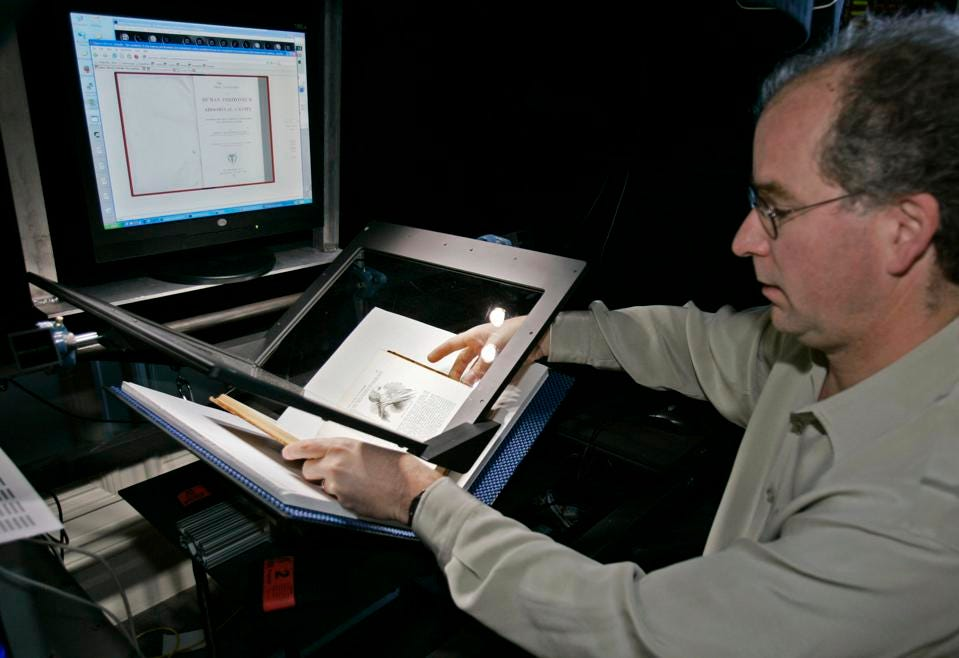
\includegraphics[width=10cm]{images/scaneandoLibro.jpg}
\end{figure} 

\begin{quote}
Goethe dijo una vez que visitar una biblioteca era como entrar en el presencia de una gran rico que silenciosamente estaba pagando dividendos incalculables
\end{quote}
\section*{ANTECEDENTES INSTITUCIONALES}
\subsubsection{Necesidades del software}
Actualmente un estudiante posee los libros digitales o digitalizados y otros como videos, artículos en un disco duro de 2 TB organizado en carpetas sin acceso fácil a ellos. En la actualidad sólo es
posible hacer un link con un programa llamano Kiwix Desktop con el cual es posible acceder con un click al libro en formato pdf o cualquier otro video o artículo o audio (aquí llamados documentos). Este método es inefectivo ya que requiere mucho tiempo para hacer los links.
Los libros están en diferentes formatos como ser: pdf, pub, djvu, pero mayormente en pdf, algunos en html. Actualmente solo se tiene en discos duros y en memoria de dispositivos móviles como tablets, celular o utro dispositivo, muchos ocupan mucha memoria porque hay redundacia de datos ya que una copia está en un disco y otra copia del mismo en otro dispositivo; sin embargo se sugiere tener una copia por si la copia descargada se corrompe.

Las videos, fueron descargados para que tengan buena calidad y sean de latencia mínima alreproducirlos, aunque no se tiene gran cantidad, pero en el futuro esto se incrementará. Los videos se tienen en discos externos; ésto para no sobrecargar el almacenamiento de la computadora personal.
Las imágenes no se tiene mucho, sin embargo como el alumno suele ser más visual en el método de aprendizaje tambien se prevee tener una base de datos de imágenes importante y relevantes a cada tema.

En otros se tiene herramientas como calculadoras, IDEs, CASE, diagramadores y páginas web relacionados con simulación y otros necesarios para aprendizaje.
\subsubsection*{Problemas por la no existencia del software}
El alumno o estudiante tiene mucha información generada durante su paso como estudiante pero éstas estan desorganizadas y el acceso a veces se vuelve de forma que no se puede encontrar lo que se busca. 

Si el alumno tiene ordenado en su computadora cuando se encuentra lejos de donde estudia, no puede acceder y debe llevar copias pero a veces copia un contenido pero tarda en copiar o simplemente copió otro contenido y un sin fin de problemas que puede tener el no accesos oportuno a la información. 

\section*{LIMITES Y ALCANCES DEL SISTEMA}
En primera instancia sólo se desarrollará para documentos tales como artículos y libros, sin embargo para versiones posteriores será extensible a cualquier objeto digital que el alumno requiera para su aprendizaje. 

\section*{JUSTIFICACIÓN}
Un usuario cualquiera requiere como soporte una colección bien articulada de información organizada y estructurada aquí llamados documentos (texto, audio, video es decir un conjunto de objetos digitales, simuladores, etc) para ayudarse un individuo a lograr un objetivo cualquiera y esto no requiere un gran espacio físico. Se quiere realizar esta biblioteca ya que la red de redes carece de caracteristicas esenciales de selección y organización a pesar que pueden existir sitios web con contenido bien organizado la libreria digital puede expandirse facilmente añadiendose nuevo material. Además no a todo el territorio boliviano alcanza la red de redes y ademas si fuera esto posible la velocidad del internet no siempre es alta y que un video pueda ser reprocucido de inmediato y sin latencia de carga y con el dificultad de que buscar algo en internet a veces suele ser como buscar en un pajar. 

Hoy en día con la revulución de la información y el poder de la tecnología hay una demanda sin precedencias para el almacenamiento, organización y acceso a la información y si la información es la moneda de la economia del conocimiento entonces las librerias digitales serán los bancos donde se invierte \cite{91364001}. 

Una biblioteca convencional o en carpetas tiene unas sola forma de organizar, mientras que en una biblioteca digital se puede organizar de diferentes maneras. 

\section*{OBJETIVOS DEL SISTEMA}
El objetivo es realizar el diseño de una herramienta de estudio efectiva para población de diferentes niveles para ayudar en el  proceso de aprendizaje.  
\section*{OBJETIVOS SECUNDARIOS}
\begin{itemize}
	\item Hacer una biblioteca digital más flexible y adaptable posible.
	\item Seleccionar organizar y mantener objetos digitales para el estudiante
\end{itemize}


